\section{Classification}

After segmentation is completed, we run classification on each segment. This is to determine the probability that a given segment is one of four types - vertex, self-loop, edge, or arrow. These probabilities are used in domain interpretation step to reconstruct the original graph. 

\subsection{Algorithm}

In order to determine the segment's probability distribution, we find five parameters. These parameters were chosen by \citeauthor{daly2015hand} \cite{daly2015hand}, based on the alpha shape and convex hull of the segment. \\ 

To compute the alpha shape and convex hull, we use the Alpha Shape Toolbox library \cite{alphashapetoolbox}, as well as SciPy's ConvexHull implementation \cite{scipy}. These libraries provide tools to easily find the area, perimeter, and points of these shapes. \\

\subsubsection{Circumscribed circle}

The first parameter is used to distinguish vertices and loops from other segments. This parameter $x_1$ is computed as \\

\begin{equation}
	x_1 = \frac{\text{Area of Convex Hull}}{\text{Area of circumscribed circle of Convex Hull}}
\end{equation} \\

The convex hull is not necessarily cyclic, so we define the circumscribed circle as a circle with diameter equal to the distance between the two farthest points in the convex hull. \\

\subsubsection{Inscribed triangle}

The second parameter is used to distinguish arrows. This parameter $x_2$ is computed as \\

\begin{equation}
	x_2 = \frac{\text{Area of largest inner triangle with angles over 20\textdegree}}{\text{Area of Convex Hull}}
\end{equation} \\

We use the method by \citeauthor{largesttriangle} \cite{largesttriangle} to find the area of the largest inner triangle.

\subsubsection{Alpha shape ratio}

The third parameter is used to distinguish line segments. This parameter $x_3$ is computed as \\

\begin{equation}
	x_3 = \frac{\text{Perimeter of alpha shape with $\alpha$ = 25}}{500 \cdot \text{Area of alpha shape with $\alpha$ = 25}}
\end{equation} \\

\subsubsection{Perimeter}

The fourth parameter is used to distinguish vertices and arrows from other segments. This parameter $x_4$ is computed as \\

\begin{equation}
	x_4 = \frac{\text{Perimeter of Convex Hull}}{\text{500}}
\end{equation} \\

\subsubsection{Disjoint shapes}

The final parameter disqualifies any strokes that are not properly segmented. This parameter $x_5$ is computed as \\

\begin{equation}
	x_5 = \text{Number of disjoint regions in alpha shape over 50 pixels apart} - 1
\end{equation} \\

The weights applied to each parameter reflect traits held by classes of stroke. For example, vertices and self-loops are almost circular, so they assign high positive weight to the circumscribed circle parameter. For testing purposes, we use the original weights trained by \citeauthor{daly2015hand} \cite{daly2015hand}. Notably, the weight for parameter $x_5$ is not trained, and instead set to always be -1000, to minimize the probability distribution of any shape with multiple disjoint regions.

\subsection{Experiments}
Similarly to the segmentation algorithm, we tested classification by drawing strokes on the iPyCanvas. One example is shown in Figure \ref{fig:classification_example}.

\subsection{Future Work}

Our future work is to connect the probability distributions computed in this step to the domain interpretation step. Certain classes tend to have similar probabilities, for example, vertices and self-loops are difficult to differentiate. These are typically differentiated in domain interpretation rather than classification. \\

In addition, we may need to further test these implementations on more data, or train more on our own data so that our weights better reflect our specific implementations.

\begin{figure}
	\centering
	\begin{subfigure}{0.9\textwidth}
		\centering
		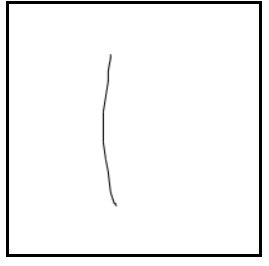
\includegraphics[scale=0.5]{./img/classificationexample}
	\end{subfigure}
	\caption{Example segment. $p_{vertex} = 0.0000076\text{, }   p_{arrow} = 0.256\text{, } p_{edge} = 0.996\text{, }  p_{loop} = 0.000086$}
	\label{fig:classification_example}
\end{figure}
